\documentclass[aspectratio=169,10pt]{beamer}

\usepackage[T1]{fontenc}
\usepackage[utf8]{inputenc}
\usepackage{lmodern}
\usepackage{tikz}
\usetikzlibrary{arrows.meta,positioning,calc}
\usepackage{xcolor}
\usepackage{listings}
\usepackage{amsmath}
\usepackage{booktabs}

\usetheme{Madrid}
\usecolortheme{seahorse}
\setbeamertemplate{navigation symbols}{}
\newcommand{\TotalFramesFixed}{42}
\setbeamertemplate{footline}{%
  \leavevmode%
  \hbox{\begin{beamercolorbox}[wd=\paperwidth,ht=2.6ex,dp=1.1ex,right]{page number in head/foot}%
    \usebeamerfont{page number in head/foot}\insertframenumber/\TotalFramesFixed\hspace*{1.5ex}
  \end{beamercolorbox}}%
}

\definecolor{pyblue}{HTML}{1F77B4}
\definecolor{pygreen}{HTML}{2CA02C}
\definecolor{pyorange}{HTML}{FF7F0E}
\definecolor{pypurple}{HTML}{9467BD}
\definecolor{pygray}{HTML}{F2F4F8}
\definecolor{dark}{HTML}{1F2937}

\lstdefinestyle{pythonstyle}{
  language=Python,
  basicstyle=\ttfamily\small,
  keywordstyle=\color{pyblue}\bfseries,
  commentstyle=\color{pygreen},
  stringstyle=\color{pyorange},
  showstringspaces=false,
  columns=fullflexible,
  keepspaces=true,
  frame=single,
  rulecolor=\color{gray!40},
  backgroundcolor=\color{pygray},
  breaklines=true
}
\lstset{style=pythonstyle}

\tikzset{
  box/.style={draw=dark, rounded corners=2mm, very thick, align=center, fill=pygray, minimum height=10mm, inner sep=2.5mm},
  bluebox/.style={box, fill=blue!12},
  greenbox/.style={box, fill=green!12},
  orangebox/.style={box, fill=orange!16},
  purplebox/.style={box, fill=purple!12},
  redbox/.style={box, fill=red!12},
  arrow/.style={-{Latex[length=2.5mm]}, very thick, draw=dark}
}

\title[Basic I/O in Python]{Basic Input/Output in Python}
\subtitle{Using \texttt{print()}, \texttt{input()}, type conversion, and f-strings}
\author{Introductory Python Programming}
\date{}

\begin{document}

\begin{frame}
  \titlepage
\end{frame}

\begin{frame}{Lesson roadmap}
\begin{enumerate}
  \item Displaying data with \texttt{print()}
  \item Receiving keyboard input with \texttt{input()}
  \item Converting input data types
  \item Input $\rightarrow$ Process $\rightarrow$ Output
  \item Formatting output with f-strings
  \item Common input/output errors
  \item Integrated practice exercises
\end{enumerate}
\end{frame}

\begin{frame}{Learning objectives}
After this lesson, students will be able to:
\begin{itemize}
  \item use \texttt{print()} to display data;
  \item print multiple values with \texttt{sep} and \texttt{end};
  \item use \texttt{input()} to receive keyboard input;
  \item explain why \texttt{input()} returns \texttt{str};
  \item convert input to \texttt{int} or \texttt{float};
  \item combine input, processing, and output in one program;
  \item format output using basic f-strings.
\end{itemize}
\begin{alertblock}{Lesson scope}
All programs are written directly with basic statements. User-defined functions (\texttt{def}) are not used yet.
\end{alertblock}
\end{frame}

\begin{frame}{The basic program pattern}
\begin{center}
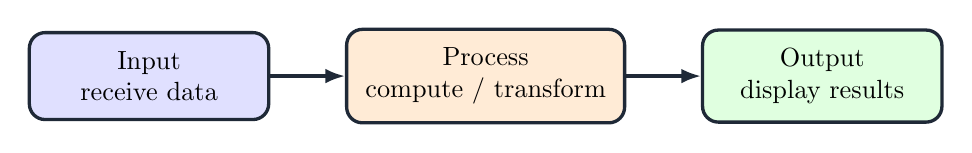
\begin{tikzpicture}[scale=0.95, every node/.style={transform shape}]
  \node[bluebox, minimum width=3.2cm] (input) at (0,0) {Input\\receive data};
  \node[orangebox, minimum width=3.2cm] (process) at (4.5,0) {Process\\compute / transform};
  \node[greenbox, minimum width=3.2cm] (output) at (9.0,0) {Output\\display results};
  \draw[arrow] (input.east) -- (process.west);
  \draw[arrow] (process.east) -- (output.west);
\end{tikzpicture}
\end{center}
\vspace{0.3cm}
\begin{block}{Example: rectangle area}
Input length and width $\rightarrow$ calculate area $\rightarrow$ display the result.
\end{block}
\end{frame}

\section{Displaying Data with print()}

\begin{frame}[fragile]{Displaying data with \texttt{print()}}
\begin{block}{Basic syntax}
\begin{lstlisting}
print(value)
\end{lstlisting}
\end{block}
\begin{exampleblock}{Example}
\begin{lstlisting}
print("Hello, Python!")
\end{lstlisting}
\end{exampleblock}
\begin{block}{Output}
\begin{verbatim}
Hello, Python!
\end{verbatim}
\end{block}
\end{frame}

\begin{frame}[fragile]{Printing numbers and variables}
\begin{columns}[T,onlytextwidth]
\column{0.48\textwidth}
\begin{block}{Numbers}
\begin{lstlisting}
print(100)
print(3.14)
\end{lstlisting}
\end{block}
\column{0.48\textwidth}
\begin{block}{Variables}
\begin{lstlisting}
name = "An"
age = 18
print(name)
print(age)
\end{lstlisting}
\end{block}
\end{columns}
\vspace{0.3cm}
\begin{alertblock}{Key idea}
\texttt{print()} can display literal values and values stored in variables.
\end{alertblock}
\end{frame}

\begin{frame}[fragile]{Printing multiple values}
\texttt{print()} can receive more than one value.
\begin{lstlisting}
name = "An"
age = 18
print("Name:", name)
print("Age:", age)
\end{lstlisting}
\begin{block}{Output}
\begin{verbatim}
Name: An
Age: 18
\end{verbatim}
\end{block}
\begin{itemize}
  \item By default, Python inserts a space between printed values.
\end{itemize}
\end{frame}

\begin{frame}[fragile]{Default separator}
\begin{lstlisting}
x = 10
y = 20
print(x, y)
\end{lstlisting}
\begin{block}{Output}
\begin{verbatim}
10 20
\end{verbatim}
\end{block}
\begin{center}
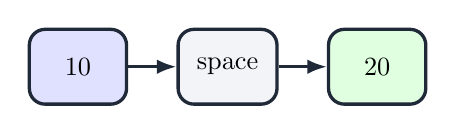
\begin{tikzpicture}[scale=0.95, every node/.style={transform shape}]
  \node[bluebox, minimum width=1.3cm] (a) at (0,0) {10};
  \node[box, minimum width=1.3cm] (space) at (2.0,0) {space};
  \node[greenbox, minimum width=1.3cm] (b) at (4.0,0) {20};
  \draw[arrow] (a) -- (space); \draw[arrow] (space) -- (b);
\end{tikzpicture}
\end{center}
\end{frame}

\begin{frame}[fragile]{The \texttt{sep} parameter}
\begin{block}{Purpose}
\texttt{sep} controls what is placed between printed values.
\end{block}
\begin{columns}[T,onlytextwidth]
\column{0.48\textwidth}
\begin{lstlisting}
print("2026", "09", "06", sep="-")
\end{lstlisting}
\begin{verbatim}
2026-09-06
\end{verbatim}
\column{0.48\textwidth}
\begin{lstlisting}
print("Python", "Java", "C++", sep=" | ")
\end{lstlisting}
\begin{verbatim}
Python | Java | C++
\end{verbatim}
\end{columns}
\end{frame}

\begin{frame}[fragile]{The \texttt{end} parameter}
\begin{block}{Default behavior}
After each \texttt{print()} statement, Python moves to a new line.
\end{block}
\begin{columns}[T,onlytextwidth]
\column{0.48\textwidth}
\begin{lstlisting}
print("Hello")
print("Python")
\end{lstlisting}
\begin{verbatim}
Hello
Python
\end{verbatim}
\column{0.48\textwidth}
\begin{lstlisting}
print("Hello", end=" ")
print("Python")
\end{lstlisting}
\begin{verbatim}
Hello Python
\end{verbatim}
\end{columns}
\end{frame}

\begin{frame}[fragile]{Self-Check 1}
\begin{block}{Question 1}
What is the output?
\begin{lstlisting}
print("A", "B", "C", sep="-")
\end{lstlisting}
\end{block}
\begin{block}{Question 2}
What is the output?
\begin{lstlisting}
print("Hello", end=" ")
print("World")
\end{lstlisting}
\end{block}
\end{frame}

\begin{frame}{Answers to Self-Check 1}
\begin{enumerate}
  \item \texttt{A-B-C}
  \item \texttt{Hello World}
\end{enumerate}
\end{frame}

\section{Receiving Input with input()}

\begin{frame}[fragile]{Receiving input with \texttt{input()}}
\begin{block}{Syntax}
\begin{lstlisting}
variable = input("Prompt")
\end{lstlisting}
\end{block}
\begin{exampleblock}{Example}
\begin{lstlisting}
name = input("Enter your name: ")
print("Hello", name)
\end{lstlisting}
\end{exampleblock}
\begin{alertblock}{Meaning}
The prompt is shown to the user. The program waits until the user types data and presses Enter.
\end{alertblock}
\end{frame}

\begin{frame}{What does \texttt{input()} do?}
\begin{center}
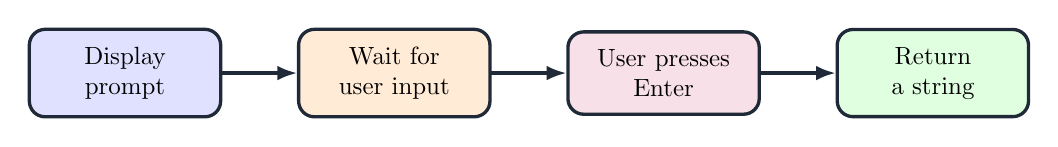
\begin{tikzpicture}[scale=0.9, every node/.style={transform shape}]
  \node[bluebox, minimum width=2.7cm] (prompt) at (0,0) {Display\\prompt};
  \node[orangebox, minimum width=2.7cm] (wait) at (3.8,0) {Wait for\\user input};
  \node[purplebox, minimum width=2.7cm] (enter) at (7.6,0) {User presses\\Enter};
  \node[greenbox, minimum width=2.7cm] (return) at (11.4,0) {Return\\a string};
  \draw[arrow] (prompt) -- (wait);
  \draw[arrow] (wait) -- (enter);
  \draw[arrow] (enter) -- (return);
\end{tikzpicture}
\end{center}
\vspace{0.3cm}
\begin{block}{Four steps}
Display a prompt, wait for input, receive the entered text, and return the text to the program.
\end{block}
\end{frame}

\begin{frame}[fragile]{\texttt{input()} returns a string}
\begin{lstlisting}
age = input("Enter your age: ")
print(type(age))
\end{lstlisting}
If the user enters \texttt{18}, the result is still:
\begin{verbatim}
<class 'str'>
\end{verbatim}
\begin{alertblock}{Important}
Even when the input looks like a number, \texttt{input()} returns data of type \texttt{str}.
\end{alertblock}
\end{frame}

\section{Converting Input Data Types}

\begin{frame}{Why type conversion is needed}
\begin{center}
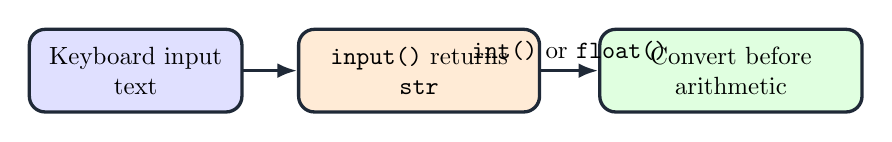
\begin{tikzpicture}[scale=0.9, every node/.style={transform shape}]
  \node[bluebox, minimum width=3.0cm] (raw) at (0,0) {Keyboard input\\text};
  \node[orangebox, minimum width=3.4cm] (str) at (4.0,0) {\texttt{input()} returns\\\texttt{str}};
  \node[greenbox, minimum width=3.7cm] (num) at (8.4,0) {Convert before\\arithmetic};
  \draw[arrow] (raw) -- (str);
  \draw[arrow] (str) -- node[above]{\texttt{int()} or \texttt{float()}} (num);
\end{tikzpicture}
\end{center}
\vspace{0.35cm}
\begin{block}{Rule}
When input data is used in arithmetic calculations, convert it to the appropriate numeric type.
\end{block}
\end{frame}

\begin{frame}[fragile]{Converting to an integer with \texttt{int()}}
\begin{lstlisting}
age = int(input("Enter your age: "))
print(age + 1)
\end{lstlisting}
If the user enters \texttt{18}, the output is:
\begin{verbatim}
19
\end{verbatim}
\begin{itemize}
  \item Use \texttt{int()} for whole numbers.
  \item Examples: age, quantity, number of students.
\end{itemize}
\end{frame}

\begin{frame}[fragile]{Converting to a floating-point number with \texttt{float()}}
\begin{lstlisting}
price = float(input("Enter price: "))
print(price)
\end{lstlisting}
\begin{itemize}
  \item Use \texttt{float()} for numbers that may contain decimals.
  \item Examples: price, height, weight, temperature.
\end{itemize}
\end{frame}

\begin{frame}[fragile]{Without type conversion}
\begin{lstlisting}
x = input("Enter x: ")
y = input("Enter y: ")
print(x + y)
\end{lstlisting}
If the user enters \texttt{10} and \texttt{20}, the output is:
\begin{verbatim}
1020
\end{verbatim}
\begin{alertblock}{Why?}
\texttt{x} and \texttt{y} are strings, so \texttt{+} concatenates them.
\end{alertblock}
\end{frame}

\begin{frame}[fragile]{With type conversion}
\begin{lstlisting}
x = int(input("Enter x: "))
y = int(input("Enter y: "))
print(x + y)
\end{lstlisting}
Output:
\begin{verbatim}
30
\end{verbatim}
\begin{alertblock}{Difference}
After conversion, \texttt{x} and \texttt{y} are integers, so \texttt{+} performs addition.
\end{alertblock}
\end{frame}

\begin{frame}[fragile]{Self-Check 2}
\begin{block}{Question 1}
What does this code print if the user enters \texttt{5}?
\begin{lstlisting}
x = input("x = ")
print(x * 3)
\end{lstlisting}
\end{block}
\begin{block}{Question 2}
How can the code be modified so that the result is \texttt{15}?
\end{block}
\end{frame}

\begin{frame}[fragile]{Answers to Self-Check 2}
\begin{enumerate}
  \item The output is \texttt{555}. The value is the string \texttt{"5"}, so multiplying by 3 repeats the string.
  \item Convert the input to an integer:
\end{enumerate}
\begin{lstlisting}
x = int(input("x = "))
print(x * 3)
\end{lstlisting}
\end{frame}

\section{Input - Process - Output}

\begin{frame}{The Input - Process - Output model}
\begin{center}
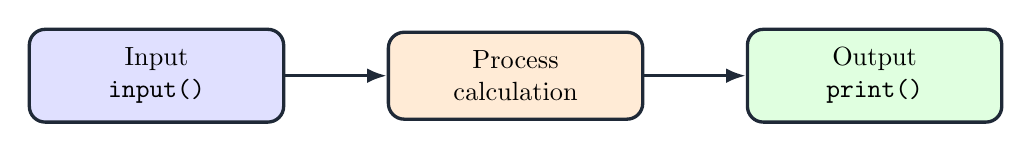
\begin{tikzpicture}[scale=0.95, every node/.style={transform shape}]
  \node[bluebox, minimum width=3.4cm] (input) at (0,0) {Input\\\texttt{input()}};
  \node[orangebox, minimum width=3.4cm] (process) at (4.8,0) {Process\\calculation};
  \node[greenbox, minimum width=3.4cm] (output) at (9.6,0) {Output\\\texttt{print()}};
  \draw[arrow] (input.east) -- (process.west);
  \draw[arrow] (process.east) -- (output.west);
\end{tikzpicture}
\end{center}
\begin{block}{Programming habit}
For beginner programs, clearly identify input, processing, and output before coding.
\end{block}
\end{frame}

\begin{frame}[fragile]{Example: rectangle area}
\begin{lstlisting}
length = float(input("Length: "))
width = float(input("Width: "))
area = length * width
print("Area:", area)
\end{lstlisting}
\begin{columns}[T,onlytextwidth]
\column{0.32\textwidth}
\begin{block}{Input}
\texttt{length}, \texttt{width}
\end{block}
\column{0.32\textwidth}
\begin{block}{Process}
\texttt{length * width}
\end{block}
\column{0.32\textwidth}
\begin{block}{Output}
\texttt{print(...)}
\end{block}
\end{columns}
\end{frame}

\section{Formatting Output with f-Strings}

\begin{frame}[fragile]{Formatting output with f-strings}
F-strings provide a clear way to combine text with variable values.
\begin{lstlisting}
name = "An"
age = 18
print(f"My name is {name}.")
print(f"I am {age} years old.")
\end{lstlisting}
\begin{block}{Output}
\begin{verbatim}
My name is An.
I am 18 years old.
\end{verbatim}
\end{block}
\end{frame}

\begin{frame}[fragile]{Expressions inside f-strings}
\begin{lstlisting}
x = 10
y = 5
print(f"{x} + {y} = {x + y}")
\end{lstlisting}
Output:
\begin{verbatim}
10 + 5 = 15
\end{verbatim}
\begin{alertblock}{Key idea}
Expressions inside \texttt{\{ \}} are evaluated before being inserted into the string.
\end{alertblock}
\end{frame}

\begin{frame}[fragile]{Formatting floating-point numbers}
\begin{lstlisting}
price = 19.5678
print(f"Price: {price:.2f}")
\end{lstlisting}
Output:
\begin{verbatim}
Price: 19.57
\end{verbatim}
\begin{block}{Meaning}
\texttt{.2f} displays a floating-point number with 2 digits after the decimal point.
\end{block}
\end{frame}

\section{Common Errors}

\begin{frame}[fragile]{Common error: forgetting type conversion}
\begin{columns}[T,onlytextwidth]
\column{0.48\textwidth}
\begin{alertblock}{Incorrect}
\begin{lstlisting}
age = input("Age: ")
next_age = age + 1
\end{lstlisting}
\end{alertblock}
\column{0.48\textwidth}
\begin{exampleblock}{Correct}
\begin{lstlisting}
age = int(input("Age: "))
next_age = age + 1
\end{lstlisting}
\end{exampleblock}
\end{columns}
\vspace{0.25cm}
\begin{block}{Reason}
\texttt{age} is a string, while \texttt{1} is an integer. They cannot be added directly.
\end{block}
\end{frame}

\begin{frame}[fragile]{Common error: invalid numeric input}
\begin{lstlisting}
age = int(input("Age: "))
\end{lstlisting}
\begin{block}{Problem}
If the user enters \texttt{eighteen}, Python cannot convert that string into an integer.
\end{block}
\begin{alertblock}{Lesson scope}
For now, assume that users enter data in the required format. Input validation will be introduced later.
\end{alertblock}
\end{frame}

\begin{frame}[fragile]{Common error: variable vs string literal}
\begin{columns}[T,onlytextwidth]
\column{0.48\textwidth}
\begin{block}{Print the text \texttt{x}}
\begin{lstlisting}
x = 10
print("x")
\end{lstlisting}
Output:
\begin{verbatim}
x
\end{verbatim}
\end{block}
\column{0.48\textwidth}
\begin{block}{Print the value of \texttt{x}}
\begin{lstlisting}
x = 10
print(x)
\end{lstlisting}
Output:
\begin{verbatim}
10
\end{verbatim}
\end{block}
\end{columns}
\end{frame}

\section{Integrated Examples}

\begin{frame}[fragile]{Integrated example 1: personal information}
\begin{lstlisting}
name = input("Name: ")
age = int(input("Age: "))

print(f"Hello {name}!")
print(f"Next year you will be {age + 1}.")
\end{lstlisting}
\begin{block}{IPO analysis}
\begin{itemize}
  \item Input: name and age
  \item Process: compute \texttt{age + 1}
  \item Output: greeting and next year's age
\end{itemize}
\end{block}
\end{frame}

\begin{frame}[fragile]{Integrated example 2: total cost}
\begin{lstlisting}
price = float(input("Product price: "))
quantity = int(input("Quantity: "))
total = price * quantity

print(f"Total: {total:.2f}")
\end{lstlisting}
\begin{block}{Important conversions}
\begin{itemize}
  \item \texttt{price}: use \texttt{float()}
  \item \texttt{quantity}: use \texttt{int()}
  \item \texttt{total}: display with \texttt{.2f}
\end{itemize}
\end{block}
\end{frame}

\begin{frame}[fragile]{Integrated example 3: Celsius to Fahrenheit}
Formula:
\[
F = \frac{9}{5}C + 32
\]
\begin{lstlisting}
celsius = float(input("Celsius: "))
fahrenheit = 9 / 5 * celsius + 32
print(f"Fahrenheit: {fahrenheit:.2f}")
\end{lstlisting}
\end{frame}

\begin{frame}[fragile]{Predict the output: exercises}
\begin{columns}[T,onlytextwidth]
\column{0.48\textwidth}
\begin{block}{Exercise 1}
\begin{lstlisting}
x = "10"
y = "5"
print(x + y)
\end{lstlisting}
\end{block}
\begin{block}{Exercise 2}
\begin{lstlisting}
x = 10
y = 5
print("Result:", x + y)
\end{lstlisting}
\end{block}
\column{0.48\textwidth}
\begin{block}{Exercise 3}
\begin{lstlisting}
print("A", "B", sep=":", end=" ")
print("C")
\end{lstlisting}
\end{block}
\begin{block}{Exercise 4}
\begin{lstlisting}
x = 7
print(f"x = {x}, x^2 = {x * x}")
\end{lstlisting}
\end{block}
\end{columns}
\end{frame}

\begin{frame}{Answers: predict the output}
\begin{enumerate}
  \item \texttt{105}
  \item \texttt{Result: 15}
  \item \texttt{A:B C}
  \item \texttt{x = 7, x\string^2 = 49}
\end{enumerate}
\end{frame}

\section{Practice Exercises}

\begin{frame}{Practice exercises 1-4}
\begin{block}{General requirement}
Write statements directly using the Input - Process - Output model. Do not use \texttt{def} yet.
\end{block}
\begin{enumerate}
  \item Greeting: input a name and display \texttt{Hello, <name>!}
  \item Age next year: input age and display next year's age.
  \item Sum and product: input two integers, then display their sum and product.
  \item Rectangle: input length and width, then display area and perimeter.
\end{enumerate}
\end{frame}

\begin{frame}{Practice exercises 5-8}
\begin{enumerate}
  \item Total purchase cost: input product name, unit price, and quantity, then display an invoice.
  \item Temperature conversion: convert Celsius to Fahrenheit and display 2 decimals.
  \item Average score: input three scores and display the average with 2 decimals.
  \item Convert seconds: input total seconds, then display full minutes and remaining seconds.
\end{enumerate}
\begin{block}{Useful operators for Exercise 8}
\texttt{//} for integer division and \texttt{\%} for remainder.
\end{block}
\end{frame}

\begin{frame}{Integrated practice: trip cost}
\begin{block}{Input}
Distance traveled, fuel consumption in liters per 100 km, and fuel price.
\end{block}
\begin{block}{Formulas}
\[
\text{fuel\_used} = \frac{\text{distance} \times \text{consumption}}{100}
\]
\[
\text{cost} = \text{fuel\_used} \times \text{fuel\_price}
\]
\end{block}
\end{frame}

\begin{frame}[fragile]{Integrated practice: sample output}
\begin{verbatim}
Distance: 250
Consumption (L/100km): 7.5
Fuel price: 23000
Fuel used: 18.75 L
Estimated cost: 431250.00
\end{verbatim}
\begin{alertblock}{Focus}
This exercise combines input, type conversion, arithmetic, and formatted output.
\end{alertblock}
\end{frame}

\begin{frame}{Self-assessment after the lesson}
\small
\begin{itemize}
  \item I know how to use \texttt{print()}.
  \item I understand \texttt{sep} and \texttt{end}.
  \item I know how to use \texttt{input()}.
  \item I remember that \texttt{input()} returns \texttt{str}.
  \item I know when to use \texttt{int()} or \texttt{float()}.
  \item I can write a program using the Input - Process - Output model.
  \item I can format floating-point values using \texttt{.2f}.
  \item I can independently write simple programs without using \texttt{def}.
\end{itemize}
\end{frame}

\begin{frame}[fragile]{Knowledge summary}
Important tools:
\begin{lstlisting}
print(...)
input(...)
int(...)
float(...)
type(...)
\end{lstlisting}
Common patterns:
\begin{lstlisting}
age = int(input("Age: "))
price = float(input("Price: "))
print(f"Result: {result:.2f}")
\end{lstlisting}
\end{frame}

\begin{frame}{Final takeaway}
\begin{center}
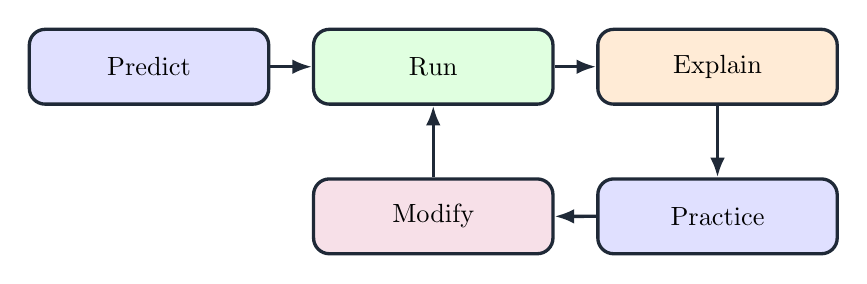
\begin{tikzpicture}[scale=0.95, every node/.style={transform shape}]
  \node[bluebox, minimum width=3.2cm] (predict) at (0,0) {Predict};
  \node[greenbox, minimum width=3.2cm] (run) at (3.8,0) {Run};
  \node[orangebox, minimum width=3.2cm] (explain) at (7.6,0) {Explain};
  \node[purplebox, minimum width=3.2cm] (modify) at (3.8,-2.0) {Modify};
  \node[bluebox, minimum width=3.2cm] (practice) at (7.6,-2.0) {Practice};
  \draw[arrow] (predict) -- (run);
  \draw[arrow] (run) -- (explain);
  \draw[arrow] (explain.south) -- (practice.north);
  \draw[arrow] (practice) -- (modify);
  \draw[arrow] (modify.north) -- (run.south);
\end{tikzpicture}
\end{center}
\begin{alertblock}{Learning process}
Predict $\rightarrow$ Run $\rightarrow$ Explain $\rightarrow$ Modify $\rightarrow$ Practice.
\end{alertblock}
\end{frame}

\end{document}
